\chapter{العصبونات وكمونات الفعل والمشابك}\label{ch:b2:neurons-synapses}

اقرع الوتر تحت الرضفة تركل الساق بعد ثلاثين
مليثانية. وفي ذلك الزمن يكون تمطط قد استُشعر في
الفخذ، وإشارة قد قطعت مترًا إلى النخاع الشوكي، وعبرت
وصلًا واحدًا إلى خلية ثانية، وقطعت مترًا راجعةً وأطلقت
تقلص عضلة --- وهي رحلة ذهاب وإياب أسرع من طرفة عين. ولا
\omterm{def:b2:cell-signalling:kinds}{هرمون} يستطيع هذا؛ وإنما تفعله خلايا مبنية للتوصيل، وإشارة
ليست مادةً تنتقل بل موجة كهرباء
تتجدد على امتداد غشاء. وهذا الفصل في تلك الخلية وتلك
الإشارة: الفولطية التي يمسكها \omterm{def:b2:neurons-synapses:neuron}{العصبون} عبر غشائه،
والدفعة التي يطلقها وكيف تسير الدفعة، \omterm{def:b2:neurons-synapses:synapse}{والمشبك} حيث
تُحوَّل الإشارة الكهربائية إلى كيميائية ثم إلى كهربائية من جديد.

\section{العصبون}

\begin{definition}[العصبون والمحوار والعصب]\label{def:b2:neurons-synapses:neuron}
\index{عصبون}\index{محوار}\index{تغصن}\index{ميالين}\index{خلية دبقية}
\emph{العصبون} خلية متخصصة للإشارة: لها جسم خلية
(\emph{سوما}) فيه النواة، و\emph{تغصنات} متفرعة
تتلقى الإشارات، و\emph{محوار} واحد --- وهو كبل من
ميكرومتر إلى عشرين ميكرومترًا ثخنًا وإلى متر طولًا ---
يحمل خرجها إلى \emph{نهايات} على خلايا أخرى. وفي
دماغ الإنسان نحو $10^{11}$ عصبون يصنع كل منها نحو
ألف \omterm{def:b2:neurons-synapses:synapse}{مشبك}. وتفوق \emph{الخلايا الدبقية} العصبونات عددًا: فالنجمية
تغذيها وتدرئ عنها، والدبقيات الصغيرة تحرسها، والخلايا
التي تلف المحاوير في \emph{الميالين} --- وهو عشرات اللفات من
غشائها هي، يكاد يخلو من الهيولى، ويؤلف غمدًا عازلًا
ينقطع كل مليمتر أو نحوه عند \emph{عقد رانفييه}.
و\emph{العصب} حزمة من آلاف المحاوير، حسية وحركية،
تجري معًا في نسيج ضام. والعصبونات لا تنقسم عند
البالغ (إلا في استثناءات قليلة)، والمحوار المقطوع عن جسمه يموت؛
فالعصبون خلية عليها أن تدوم عمرًا كاملًا.
\end{definition}

\begin{omfigure}
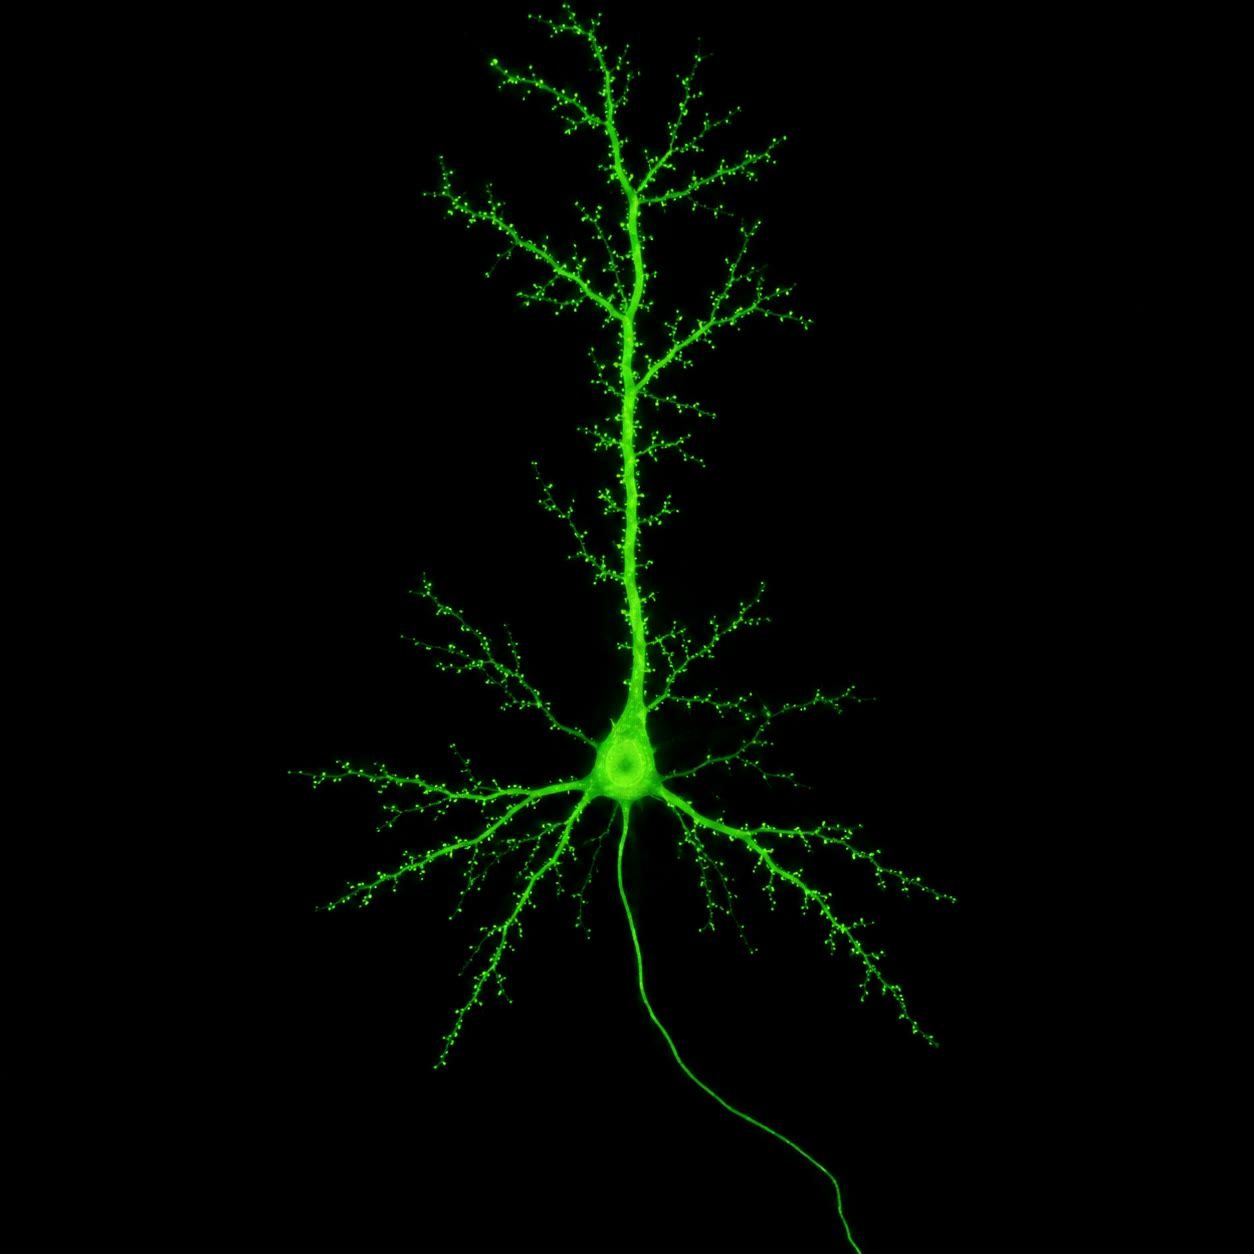
\includegraphics[width=0.4\linewidth]{images/book4/ai/b4-20-neuron-fluorescence.jpg}\hspace{0.05\linewidth}
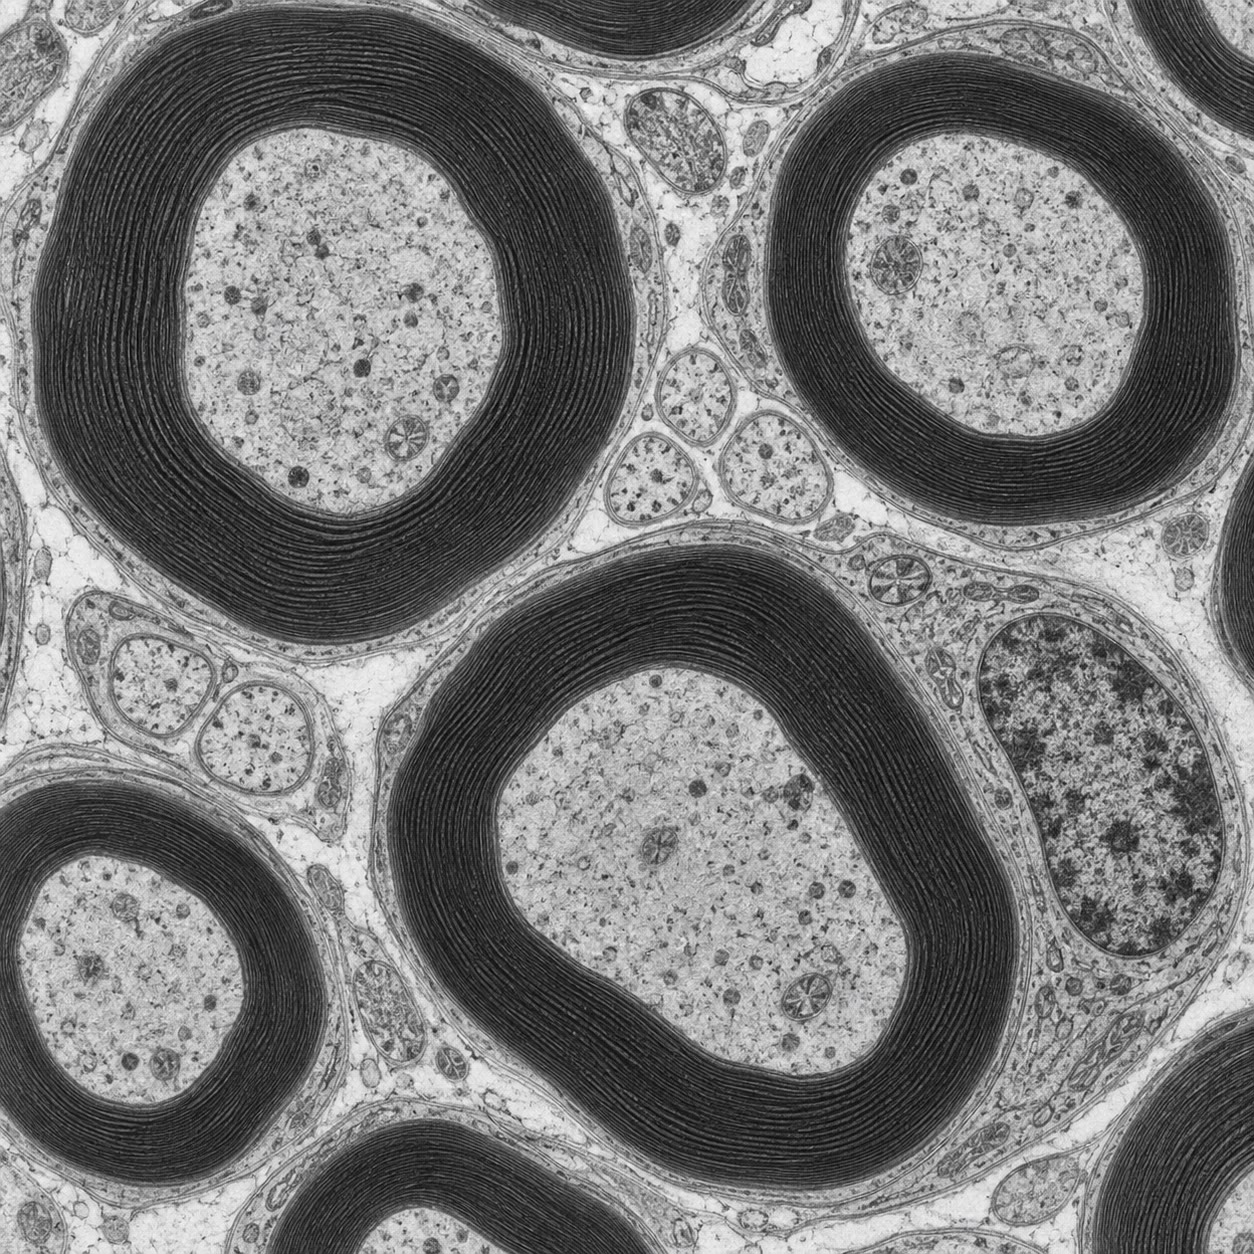
\includegraphics[width=0.4\linewidth]{images/book4/ai/b4-20-myelinated-axons-tem.jpg}

{\small إلى اليسار: \omterm{def:b2:neurons-synapses:neuron}{عصبون} هرمي مملوء بصباغ --- جسم الخلية،
والتغصنات الشوكية التي تتلقى، \omterm{def:b2:neurons-synapses:neuron}{والمحوار} الرفيع الذي يغادر
من القاعدة. وإلى اليمين: محاوير في مقطع عرضي تحت المجهر الإلكتروني،
كل منها ملفوف في حلزون داكن من غمد ميالينه.}
\end{omfigure}

\section{كمون الراحة}

\begin{theorem}[كمون نرنست]\label{thm:b2:neurons-synapses:nernst}
\index{كمون نرنست}\index{كمون التوازن}
الغشاء النفوذ لشاردة واحدة شحنتها $z$ ويفصل بين
تركيزين $c_{\text{خارج}}$ و$c_{\text{داخل}}$ يستقر عند
\emph{\omterm{thm:b2:neurons-synapses:nernst}{كمون التوازن}} الذي تتوازن عنده القوة الكهربائية على
الشاردة مع انتشارها:
\[
E = \frac{RT}{zF}\ln\frac{c_{\text{خارج}}}{c_{\text{داخل}}} \approx \frac{\qty{61.5}{mV}}{z}\log_{10}\frac{c_{\text{خارج}}}{c_{\text{داخل}}} \quad (\qty{37}{\celsius}).
\]
يمسك \omterm{def:b2:neurons-synapses:neuron}{العصبون} \qty{140}{mmol/L} من البوتاسيوم في الداخل في مقابل
\qty{5}{mmol/L} في الخارج، و\qty{15}{mmol/L} من الصوديوم في الداخل
في مقابل \qty{145}{mmol/L} في الخارج، وهي تدرجات تبنيها
مضخة الصوديوم والبوتاسيوم بثلث ATP الخلية.
ومن ثم $E_{\mathrm K} = 61.5\log_{10}(5/140) = \qty{-89}{mV}$ و
$E_{\mathrm{Na}} = 61.5\log_{10}(145/15) = \qty{+61}{mV}$: فلو لم يمرر
الغشاء غير البوتاسيوم لاستقر عند
\qty{-89}{mV}، ولو لم يمرر غير الصوديوم لاستقر عند \qty{+61}{mV}.
\end{theorem}
\begin{proof}
عند التوازن يكون الكمون الكهركيميائي للشاردة واحدًا
على الجهتين: $RT\ln c_{\text{داخل}} + zFV_{\text{داخل}} = RT\ln
c_{\text{خارج}} + zFV_{\text{خارج}}$، ومن ثم $V_{\text{داخل}} -
V_{\text{خارج}} = (RT/zF)\ln(c_{\text{خارج}}/c_{\text{داخل}})$. وعند
\qty{310}{K} يكون $RT/F = \qty{26.7}{mV}$ و$\ln 10 \times 26.7 =
\qty{61.5}{mV}$. (وقد اشتُق في مجلد السنة الأولى من توزيع
بولتزمان؛ ويُعاد ذكره هنا.)
\end{proof}

\begin{theorem}[كمون الراحة متوسطًا موزونًا]\label{thm:b2:neurons-synapses:chord}
\index{كمون الراحة}\index{ناقلية (غشاء)}
إذا كان الغشاء يوصّل عدة شوارد، لكل منها ناقلية $g_i$
(أي سهولة مرورها، وتقررها عدة القنوات المفتوحة)،
كان الكمون المستقر الذي تتلاشى عنده التيارات
\[
V = \frac{\sum_i g_i E_i}{\sum_i g_i},
\]
وهو متوسط لكمونات التوازن موزون بالناقليات.
وفي الراحة يكون غشاء \omterm{def:b2:neurons-synapses:neuron}{العصبون} أنفذ للبوتاسيوم نحو عشرين ضعفًا
منه للصوديوم، فيكون $V \approx (20\times(-89) +
61)/21 = \qty{-82}{mV}$؛ وبحساب الكلور والتسربات
الصغيرة يكون \omterm{thm:b2:neurons-synapses:chord}{كمون الراحة} \qty{-70}{mV}. ويستقر الغشاء
قرب $E_{\mathrm K}$ لأن قنوات البوتاسيوم مفتوحة؛ وكل ما يفتح
قنوات الصوديوم يجره نحو $E_{\mathrm{Na}}$ --- وذلك
هو مبدأ الإشارة العصبية كله.
\end{theorem}
\begin{proof}
تحمل كل شاردة تيارًا $I_i = g_i(V - E_i)$ (وهو قانون أوم، مع
قياس القوة الدافعة من توازن الشاردة نفسها). وعند
كمون مستقر يكون التيار الكلي صفرًا: $\sum_i g_i(V - E_i) =
0$، ومن ثم $V\sum g_i = \sum g_iE_i$. (والمعالجة التامة، التي
تدخل فيها النفوذيات عبر معادلة غولدمان--هودجكن--كاتز،
تعطي الوزن نفسه بالتقريب الأول.)
\end{proof}

\section{كمون الفعل}

\begin{proposition}[الدفعة]\label{prop:b2:neurons-synapses:ap}
\index{كمون الفعل}\index{قناة فولطية البوابة}\index{عتبة}\index{فترة حرنة}
يحمل غشاء \omterm{def:b2:neurons-synapses:neuron}{المحوار} \emph{قنوات صوديوم فولطية البوابة}، مغلقة
في الراحة ويفتحها زوال الاستقطاب. فإذا رفع منبه
الكمون من \qty{-70}{mV} فوق \emph{عتبة} قرب
\qty{-55}{mV}، انفتح منها ما يكفي لإدخال صوديوم أكثر مما
يستطيع تسرب البوتاسيوم موازنته؛ فيرتفع الكمون، وتنفتح قنوات أكثر،
وفي جزء من مليثانية يُكتسح الغشاء نحو
$E_{\mathrm{Na}}$ --- وهي \emph{تغذية راجعة موجبة} متفجرة
ولا تقبل التدرج. ويبلغ الذروة قرب \qty{+40}{mV} لأن قنوات
الصوديوم \emph{تُعطَّل} في غضون مليثانية من انفتاحها ولأن
\emph{قنوات بوتاسيوم فولطية البوابة} أبطأ تنفتح
فتعيد الكمون نحو $E_{\mathrm K}$، متجاوزةً إلى
\emph{هبوط دون الراحة} قبل أن تنغلق قنوات البوتاسيوم. ويدوم
\emph{\omterm{prop:b2:neurons-synapses:ap}{كمون الفعل}} نحو مليثانية؛ ولمليثانية أخرى
أو اثنتين لا تستطيع قنوات الصوديوم المعطَّلة أن تنفتح من جديد
(وهي \emph{\omterm{prop:b2:neurons-synapses:ap}{الفترة الحرنة}})، وذلك يحد معدل الإطلاق ببضع
مئات في الثانية ويرغم الدفعة على السير في اتجاه واحد.
ولأنها لا تقبل التدرج، لا تحمل الدفعة معلومة في
حجمها: \omterm{def:b2:neurons-synapses:neuron}{فالعصبون} يرمّز الشدة \emph{بتواترها}. ويدخل نحو
$10^{4}$ شاردة صوديوم ويخرج مثلها من البوتاسيوم في كل
دفعة --- وهو تغير مهمل في التركيز، تعيده
المضخة على مهل.
\end{proposition}
\begin{proof}[شواهد]
فصل هودجكن وهكسلي (1952)، باستعمال \omterm{def:b2:neurons-synapses:neuron}{محوار} الحبار العملاق (نصف
مليمتر ثخنًا، حتى يمكن إدخال سلك فيه) ومضخم
ذي تغذية راجعة يمسك كمون الغشاء عند أي قيمة
مختارة (وهو \emph{قامط الفولطية}) مع تسجيل التيار اللازم
لإمساكه، فصلا التيار إلى مركّبة داخلة مبكرة
تزول إذا نُزع الصوديوم من الحمّام، ومركّبة خارجة
متأخرة يحملها البوتاسيوم؛ وقاسا كيف ترتفع كل
ناقلية وتهبط مع الزمن عند كل فولطية؛ وبملاءمة
كل منهما ببضع معادلات حسبا شكل \omterm{prop:b2:neurons-synapses:ap}{كمون الفعل}
وعتبته وسرعته وفترته الحرنة من الناقليتين
وحدهما. وصدقت كل تنبؤاتهما. ورُئيت القنوات نفسها
بعد ذلك بخمس وعشرين سنة، واحدة واحدة، بقامط الرقعة؛
والتترودوتوكسين (سم السمكة المنتفخة) يحصر قناة الصوديوم
ويلغي الدفعة، ورباعي إيثيل الأمونيوم يحصر قناة
البوتاسيوم فيطيلها.
\end{proof}

\begin{omfigure}
\begin{tikzpicture}
\begin{axis}[
  width=0.9\linewidth, height=6.4cm,
  axis x line=bottom, axis y line=left,
  xmin=0, xmax=4, ymin=-100, ymax=60,
  xlabel={الزمن (ms)}, ylabel={كمون الغشاء (mV)},
  xlabel style={font=\small, at={(axis description cs:0.5,-0.1)}, anchor=north},
  ylabel style={font=\small},
  tick label style={font=\small}, xtick={0,1,2,3,4}, ytick={-90,-70,-55,0,40},
  legend style={font=\scriptsize, at={(0.97,0.95)}, anchor=north east, draw=none},
  clip=false,
]
\addplot[very thick, omDef] coordinates {(0,-70) (0.4,-70) (0.5,-64) (0.6,-55) (0.7,-30) (0.8,10) (0.9,35) (1.0,40) (1.1,30) (1.2,10) (1.35,-20) (1.5,-50) (1.7,-75) (1.9,-85) (2.2,-82) (2.6,-76) (3.2,-71) (4,-70)};
\addlegendentry{كمون الغشاء}
\addplot[thick, omThm, dashed] coordinates {(0,0) (0.5,0) (0.6,5) (0.7,20) (0.8,35) (0.9,30) (1.0,20) (1.1,8) (1.2,3) (1.4,0) (4,0)};
\addlegendentry{$g_{\mathrm{Na}}$ (نسبيًا)}
\addplot[thick, omProp, dashed] coordinates {(0,0) (0.6,0) (0.8,2) (1.0,8) (1.2,16) (1.4,20) (1.7,17) (2.0,10) (2.4,4) (3.0,1) (4,0)};
\addlegendentry{$g_{\mathrm K}$ (نسبيًا)}
\draw[dashed, gray] (axis cs:0,-55) -- (axis cs:4,-55); \node[font=\scriptsize, anchor=south east] at (axis cs:4,-55) {العتبة};
\draw[dashed, gray] (axis cs:0,-89) -- (axis cs:4,-89); \node[font=\scriptsize, anchor=south east] at (axis cs:3.7,-89) {$E_{\mathrm K}$};
\draw[<->, gray] (axis cs:1.0,50) -- (axis cs:2.5,50); \node[font=\scriptsize, anchor=south, gray] at (axis cs:1.75,50) {الفترة الحرنة};
\end{axis}
\end{tikzpicture}

{\small كمون فعل. فوق العتبة ترتفع ناقلية الصوديوم
(الحمراء) ارتفاعًا متفجرًا وتجر الكمون نحو
$E_{\mathrm{Na}}$؛ ثم تُعطَّل إذ ترتفع ناقلية البوتاسيوم
(البرتقالية) فتعيد الغشاء نحو $E_{\mathrm K}$، مع
هبوط دون الراحة. وتحت خط العتبة لا يحدث شيء.}
\end{omfigure}

\section{التوصيل}

\begin{theorem}[الكبل وثابت طوله]\label{thm:b2:neurons-synapses:cable}
\index{ثابت الطول}\index{معادلة الكبل}\index{سرعة التوصيل}
\omterm{def:b2:neurons-synapses:neuron}{المحوار} كبل راشح: فالتيار المحقون عند نقطة يجري على امتداد
الهيولى (بمقاومة $r_i$ لوحدة الطول) ويرشح خارجًا
عبر الغشاء (بمقاومة $r_m$ في وحدة الطول). وزوال استقطاب
مستقر مقداره $V_0$ عند $x = 0$ يخبو على امتداد \omterm{def:b2:neurons-synapses:neuron}{المحوار} هكذا
\[
V(x) = V_0\,e^{-x/\lambda}, \qquad \lambda = \sqrt{\frac{r_m}{r_i}} = \sqrt{\frac{R_m\,d}{4R_i}},
\]
حيث $d$ القطر، و$R_m$ و$R_i$ المقاومتان النوعيتان للغشاء
وللهيولى. و\emph{\omterm{thm:b2:neurons-synapses:cable}{ثابت الطول}}
$\lambda$ هو المسافة التي تهبط على مداها إشارة سلبية إلى
الثلث: وهو نحو \qty{0.5}{mm} \omterm{def:b2:neurons-synapses:neuron}{لمحوار} قطره \qty{1}{\micro m}، وينمو
كالجذر التربيعي للقطر. وتنتشر دفعة \omterm{prop:b2:neurons-synapses:ap}{كمون الفعل}
لأن زوال الاستقطاب عند جبهتها، إذ ينتشر سلبيًا إلى الأمام
بمقدار $\lambda$ نحوًا، يبلغ بالقطعة التالية من الغشاء
العتبة، فتجدده بكامل حجمه؛ وكلما بلغ أبعد
كانت الموجة أسرع، فتنمو \omterm{thm:b2:neurons-synapses:cable}{سرعة التوصيل} أيضًا
كالجذر $\sqrt{d}$ تقريبًا --- من \qty{1}{m/s} في ليف رفيع
بلا \omterm{def:b2:neurons-synapses:neuron}{ميالين} إلى \qty{20}{m/s} في \omterm{def:b2:neurons-synapses:neuron}{محوار} الحبار العملاق.
\end{theorem}
\begin{proof}
ليكن $i(x)$ التيار المحوري و$V(x)$ زوال استقطاب
الغشاء. فقانون أوم على امتداد هيولى \omterm{def:b2:neurons-synapses:neuron}{المحوار} يعطي $\mathrm{d}V/
\mathrm{d}x = -r_i\,i$؛ وحفظ الشحنة، مع الرشح عبر
الغشاء، يعطي $\mathrm{d}i/\mathrm{d}x = -V/r_m$. وبالجمع بينهما
يكون $\mathrm{d}^{2}V/\mathrm{d}x^{2} = V/(r_m r_i)$، وحله
الخابي هو $V_0 e^{-x/\lambda}$ مع $\lambda^{2} = r_m/r_i$. ولأسطوانة
يكون $r_m = R_m/(\pi d)$ و$r_i = 4R_i/(\pi d^{2})$، ومن ثم
$\lambda^{2} = R_m d/4R_i$. وعند $R_m = \qty{1}{\ohm.m^2}$ و$R_i =
\qty{1}{\ohm.m}$ و$d = \qty{1}{\micro m}$: $\lambda = \sqrt{10^{-6}
/4} = \qty{0.5}{mm}$.
\end{proof}

\begin{proposition}[الميالين والتوصيل القفزي]\label{prop:b2:neurons-synapses:myelin}
\index{توصيل قفزي}\index{عقدة رانفييه}
يضرب \omterm{def:b2:neurons-synapses:neuron}{الميالين} $r_m$ في عدد لفات الغشاء ويقسم
سعة الغشاء على العامل نفسه، حتى لا يكاد يرشح تحت
الغمد أي تيار ولا يلزم إلا شحنة قليلة
لتغيير الكمون: فينتشر زوال الاستقطاب سلبيًا على امتداد
قطعة بين عقدتين طولها مليمتر بفقد قليل، ولا يتجدد \omterm{prop:b2:neurons-synapses:ap}{كمون
الفعل} إلا عند العقد، حيث تتركز قنوات الصوديوم.
وهكذا \emph{تقفز} الدفعة من عقدة إلى عقدة
(وهو \emph{\omterm{prop:b2:neurons-synapses:myelin}{التوصيل القفزي}})، عند \qty{100}{m/s} في ليف
قطره \qty{20}{\micro m} --- وهي سرعة كان على \omterm{def:b2:neurons-synapses:neuron}{محوار} بلا \omterm{def:b2:neurons-synapses:neuron}{ميالين}
أن يكون ثخنه سنتيمترات ليبلغها --- وبكسر من
الكلفة الاستقلابية، إذ لا يدخل الصوديوم إلا عند العقد. \omterm{def:b2:neurons-synapses:neuron}{والميالين}
هو ابتكار الفقاريات الذي أتاح جملة عصبية كبيرة سريعة
في جسم صغير؛ وفي التصلب المتعدد يُتلف الغمد رقعةً رقعة،
فينهار \omterm{thm:b2:neurons-synapses:cable}{ثابت الطول}، وتخفق الدفعات.
\end{proposition}

\begin{omfigure}
\begin{tikzpicture}[every node/.style={font=\scriptsize}, >=stealth]
  % unmyelinated
  \begin{scope}
    \draw[thick, fill=omDef!10] (0,0) rectangle (11,0.5);
    \foreach \x in {0.5,1.0,...,10.5} \draw[omThm, ->] (\x,0.25) -- (\x,0.9);
    \node[anchor=east] at (-0.2,0.25) {بلا ميالين};
    \node[anchor=west] at (11.2,0.25) {\qty{1}{m/s}};
    \node[above] at (5.5,1.0) {تتجدد الدفعة عند كل نقطة};
  \end{scope}
  % myelinated
  \begin{scope}[yshift=-2.4cm]
    \draw[thick, fill=omDef!10] (0,0) rectangle (11,0.5);
    \foreach \x in {0.3,2.5,4.7,6.9,9.1} \fill[omExo!60] (\x,-0.15) rectangle (\x+1.9,0.65);
    \foreach \x in {2.35,4.55,6.75,8.95} \draw[omThm, ->] (\x,0.25) -- (\x,0.9);
    \foreach \x in {2.35,4.55,6.75} \draw[->, thick, omThm, dashed] (\x+0.1,1.1) .. controls (\x+1.1,1.6) .. (\x+2.1,1.1);
    \node[anchor=east] at (-0.2,0.25) {بميالين};
    \node[anchor=west] at (11.2,0.25) {\qty{100}{m/s}};
    \node[below] at (1.25,-0.2) {قطعة ميالين بين عقدتين};
    \node[below] at (4.55,-0.2) {عقدة رانفييه};
    \node[above] at (5.5,1.6) {لا تتجدد إلا عند العقد: توصيل قفزي};
  \end{scope}
\end{tikzpicture}

{\small التوصيل \omterm{def:b2:neurons-synapses:neuron}{بميالين} وبلا \omterm{def:b2:neurons-synapses:neuron}{ميالين}. في \omterm{def:b2:neurons-synapses:neuron}{المحوار} العاري تتجدد
الدفعة على امتداده كله؛ وتحت \omterm{def:b2:neurons-synapses:neuron}{الميالين} تنتشر الإشارة
سلبيًا على امتداد كل قطعة بين عقدتين وتتجدد عند العقد، فتسير
الدفعة أسرع مئة مرة.}
\end{omfigure}

\section{المشبك}

\begin{definition}[المشابك الكيميائية والكهربائية]\label{def:b2:neurons-synapses:synapse}
\index{مشبك}\index{ناقل عصبي}\index{كمون تالٍ للمشبك}
عند \emph{المشبك} تلاقي نهايةُ \omterm{def:b2:neurons-synapses:neuron}{عصبون} هدفًا --- عصبونًا
آخر، أو ليفًا عضليًا، أو خلية غدية. وفي المشبك \emph{الكهربائي}
تصل الوصلات الفجوية بين الخليتين ويمر التيار مباشرةً
--- سريعًا، ثنائي الاتجاه، بلا تضخيم، ويُستعمل حيث تهم السرعة
والتزامن (منعكسات الهرب، \omterm{def:b2:heart:anatomy}{والقلب}). أما في المشبك \emph{الكيميائي}
فتفصل بين الخليتين شق عرضه \qty{20}{nm} وتكون
الإشارة جزيئًا. فكمون فعل يصل إلى النهاية
يفتح قنوات كالسيوم فولطية البوابة؛ فيدخل الكالسيوم ويجعل، في
جزء من مليثانية، حويصلات \emph{الناقل العصبي}
تندمج مع الغشاء وتفرغ في الشق؛ وينتشر الناقل
عبره في ميكروثوان ويرتبط بمستقبلات على الغشاء
التالي للمشبك --- إما قنوات شاردية يفتحها
(\emph{شاردية التوجه}، سريعة) أو مستقبلات مقترنة \omterm{prop:b2:cell-signalling:gpcr}{ببروتين G}
(\emph{استقلابية التوجه}، أبطأ، \cref{ch:b2:cell-signalling})؛
فيزيح التيار الناتج الكمونَ التالي للمشبك بضعة
مليفولط، صعودًا (وهو \emph{كمون تالٍ للمشبك منبّه}، من
قنوات تمرر الصوديوم) أو نزولًا (وهو \emph{مثبّط}، من
قنوات تمرر الكلور أو البوتاسيوم)؛ ويُزال الناقل
في غضون مليثوان بإنزيم أو بناقل. والتأخر
نصف مليثانية؛ والثمن يشتري نقلًا في اتجاه واحد،
وتضخيمًا، وتثبيطًا، وقابلية للتعديل --- وهو كل ما تحتاجه جملة
عصبية فوق مجرد التوصيل.
\end{definition}

\begin{omfigure}
\begin{tikzpicture}[every node/.style={font=\scriptsize}, >=stealth]
  % presynaptic terminal
  \draw[thick, fill=omDef!10] (0,0) .. controls (0,2.6) and (3.6,2.6) .. (3.6,0.2) -- (3.6,-0.2) .. controls (3.6,-2.6) and (0,-2.6) .. (0,0);
  \draw[very thick, omDef] (-2.2,0) -- (0.1,0); \node[omDef, above] at (-1.1,0.05) {محوار};
  \foreach \p in {(2.0,1.0),(2.6,0.5),(2.7,-0.4),(2.1,-1.0),(1.6,0.2)} \draw[thick, fill=omProp!40] \p circle (0.25);
  \draw[thick, fill=omProp!40] (3.3,0.1) arc (90:-90:0.25) -- cycle;
  \foreach \p in {(3.75,0.2),(3.85,-0.1),(3.7,-0.35),(3.9,0.4)} \fill[omProp] \p circle (0.05);
  \fill[omThm] (3.45,1.3) circle (0.06); \node[omThm, anchor=east] at (3.35,1.45) {دخول Ca$^{2+}$};
  \draw[->, omThm] (3.9,1.5) -- (3.55,1.35);
  % cleft
  \node[align=center, anchor=north] at (3.85,-2.75) {الشق\\\qty{20}{nm}};
  \draw[gray] (3.85,-2.7) -- (3.85,-1.2);
  % postsynaptic
  \draw[thick, fill=omExo!15] (4.1,-2.6) rectangle (8.2,2.6);
  \foreach \y in {0.9,0.3,-0.3,-0.9} \draw[thick, fill=omDef!40] (4.05,\y-0.15) rectangle (4.45,\y+0.15);
  \node[anchor=west, align=left] at (4.6,0.3) {مستقبلات: قنوات\\تنفتح، وشوارد تجري،\\وكمون تالٍ\\للمشبك};
  \node[anchor=west, align=left] at (4.6,-1.7) {يُزال الناقل\\بإنزيم أو\\بناقل};
  \node[anchor=west] at (4.6,2.2) {الخلية التالية للمشبك};
  % labels
  \node[align=center, anchor=north] at (1.8,-2.75) {حويصلات\\الناقل};
  \node[anchor=south] at (1.8,2.75) {النهاية السابقة للمشبك};
\end{tikzpicture}

{\small \omterm{def:b2:neurons-synapses:synapse}{مشبك} كيميائي. الدفعة تُدخل الكالسيوم، فتندمج الحويصلات
وتطلق الناقل في الشق، وتفتح المستقبلات على
الهدف قنوات، ويُزال الناقل في غضون
مليثوان.}
\end{omfigure}

\begin{theorem}[الإطلاق الكمومي]\label{thm:b2:neurons-synapses:quantal}
\index{إطلاق كمومي}\index{كمون مصغر}
يُطلق الناقل رزمًا --- \emph{كمومات}، كل منها حويصل
واحد --- وعدد $k$ ما يطلقه دفعة واحدة متغير
عشوائي. فإذا كان في النهاية $n$ موقع إطلاق يطلق كل منها
باحتمال $p$، وكان $p$ صغيرًا، كان $k$ بواسونيًا تقريبًا
بمتوسط $m = np$:
\[
P(k) = \frac{m^{k}e^{-m}}{k!}, \qquad P(0) = e^{-m}, \qquad
m = \ln\frac{\text{عدد المحاولات}}{\text{عدد الإخفاقات}}.
\]
ومن ثم يمكن قراءة المحتوى الكمومي المتوسط $m$ من
كسر الدفعات التي لا تطلق شيئًا، والتحقق منه بقسمة
الاستجابة المتوسطة على حجم كموم واحد. وعند
\omterm{prop:b2:neurons-synapses:integration}{الوصل العصبي العضلي} يكون $m$ بضع مئات --- فلا يخفق النقل أبدًا؛
وعند \omterm{def:b2:neurons-synapses:synapse}{مشبك} مركزي يكون كثيرًا قرب الواحد، وينقل \omterm{def:b2:neurons-synapses:synapse}{المشبك}
على كسر من الدفعات.
\end{theorem}
\begin{proof}
مع $n$ موقعًا مستقلًا يطلق كل منها باحتمال $p$، يكون $k$
ثنائي الحد؛ ولأجل $n$ كبير و$p$ صغير مع بقاء $np = m$ ثابتًا،
يؤول الثنائي إلى قانون بواسون (وهو في سلسلة الرياضيات، السنة الثانية).
و$P(0) = e^{-m}$ يعطي $m$ من الإخفاقات. وتحقُّق كاتز هو أن
$m$ نفسه، إذا وُضع في صيغة بواسون، يتنبأ بالكسور الملحوظة
من الاستجابات ذات الكموم الواحد والاثنين والثلاثة.
\end{proof}
\begin{proof}[شواهد]
سجّل فات وكاتز (1952) من ليف عضلي لضفدع في الراحة
زوالات استقطاب عفوية صغيرة قدرها نحو \qty{0.5}{mV}، كلها
بالحجم نفسه، على فترات عشوائية --- وهي \emph{كمونات الصفيحة
الانتهائية المصغرة}، كل منها أثر حويصل واحد. وخفض الكالسيوم في
الحمّام قلّل الاستجابة لتنبيه العصب حتى صارت
تتذبذب بين 0 و1 و2 و3 أمثال من الحجم المصغر؛
وتبعت تواترات الأمثال قانونَ بواسون مع
$m$ المحسوب من الإخفاقات. وهكذا بيّن دل كاستيو وكاتز
أن \omterm{thm:b2:neurons-synapses:quantal}{الإطلاق كمومي}، وأن الكالسيوم يتحكم في احتمال
الإطلاق لا في حجم الكموم، وأظهر المجهر الإلكتروني
الحويصلات التي هي الكمومات.
\end{proof}

\begin{proposition}[التكامل: العصبون قرارًا]\label{prop:b2:neurons-synapses:integration}
\index{تجميع}\index{ربوة المحوار}\index{وصل عصبي عضلي}
يتلقى \omterm{def:b2:neurons-synapses:neuron}{العصبون} المركزي آلاف المشابك، منبِّهة
ومثبِّطة، على تغصناته وجسمه. وكل \omterm{def:b2:neurons-synapses:synapse}{كمون تالٍ للمشبك}
صغير يخبو سلبيًا، بثابت طول الكبل في
المكان وبثابت زمن الغشاء (بضع مليثوان) في
الزمن؛ وهي تتجمع --- \emph{تجميعًا مكانيًا} لدخلات تصل
معًا، و\emph{تجميعًا زمانيًا} لدخلات تصل في تعاقب
سريع --- ويُقرأ المجموع عند \emph{\omterm{prop:b2:neurons-synapses:integration}{ربوة المحوار}}، حيث
تكون قنوات الصوديوم أكثف والعتبة أخفض. فإن تجاوز
المجموع العتبة انطلق \omterm{def:b2:neurons-synapses:neuron}{المحوار}، بمعدل يرتفع مع
الفائض؛ والدخلات المثبطة تطرح، \omterm{def:b2:neurons-synapses:synapse}{والمشبك} المثبط القريب
من الربوة يستطيع نقض \omterm{def:b2:neurons-synapses:synapse}{مشبك} منبّه بعيد. و
\omterm{prop:b2:neurons-synapses:integration}{الوصل العصبي العضلي} هو الاستثناء الذي يبيّن القاعدة: فنهاية
حركية واحدة، تطلق مئات الكمومات من الأستيل كولين على
مستقبلات هي نفسها القنوات، تعطي كمون صفيحة انتهائية
قدره \qty{50}{mV}، وهو فوق العتبة بكثير --- فكل دفعة في العصب
الحركي تنتج كمون فعل عضليًا
(\cref{ch:b2:muscle-movement}). والكورار، الذي يحصر المستقبل،
يشل؛ والغازات العصبية، التي تحصر الإنزيم الذي يزيل
الأستيل كولين، تشل بالفائض المعاكس.
\end{proposition}

\begin{example}[النواقل والأدوية]\label{ex:b2:neurons-synapses:transmitters}
الأستيل كولين عند \omterm{prop:b2:neurons-synapses:integration}{الوصل العصبي العضلي} وفي الجملة
الذاتية؛ والغلوتامات، وهي الناقل المنبّه الرئيس في الدماغ،
وGABA، وهو المثبط الرئيس؛ والأمينات الأحادية: النورأدرينالين
والدوبامين والسيروتونين، وهي تعدّل دارات كاملة انطلاقًا من بضعة
آلاف من الخلايا؛ وعشرات الببتيدات. ويكاد كل دواء يفعل
في النفس أن يفعل في \omterm{def:b2:neurons-synapses:synapse}{مشبك}: فالبنزوديازيبينات تقوّي قناة
GABA، ومضادات الاكتئاب تحصر ناقل السيروتونين، والكوكايين
يحصر ناقل الدوبامين، والأفيونيات تحاكي ببتيدًا، والنيكوتين يحاكي
الأستيل كولين على مستقبل والأتروبين يحصره على آخر،
وذيفان الوشيقية يقطع البروتينات التي تدمج الحويصل. \omterm{def:b2:neurons-synapses:synapse}{فالمشبك}
هو حيث تلتقي كيمياء \cref{ch:b2:cell-signalling} مع
كهرباء هذا الفصل، وحيث تتعلم جملة عصبية:
فالمشابك المستعملة تقوى، وذلك التقوي (في
مجلد السنة الثالثة) هو الذاكرة.
\end{example}

\section{تمارين}

\begin{exercise}[$\star$]\label{exo:b2:neurons-synapses:1}
سمِّ أجزاء \omterm{def:b2:neurons-synapses:neuron}{العصبون} ووظيفة كل جزء، وقل مم
يتألف \omterm{def:b2:neurons-synapses:neuron}{الميالين} وماذا يفعل.
\end{exercise}

\begin{exercise}[$\star$]\label{exo:b2:neurons-synapses:2}
صف أطوار \omterm{prop:b2:neurons-synapses:ap}{كمون الفعل} وأحداث القنوات
التي تسبب كل طور. ولماذا لا يقبل التدرج، ولماذا لا يسير
راجعًا؟
\end{exercise}

\begin{exercise}[$\star$]\label{exo:b2:neurons-synapses:3}
اذكر خطوات النقل عند \omterm{def:b2:neurons-synapses:synapse}{مشبك} كيميائي من
وصول الدفعة إلى إزالة الناقل.
\end{exercise}

\begin{exercise}[$\star$]\label{exo:b2:neurons-synapses:4}
قارن بين المشابك الكهربائية والكيميائية في السرعة والاتجاه
والتضخيم وإمكان التثبيط.
\end{exercise}

\begin{exercise}[$\star\star$]\label{exo:b2:neurons-synapses:5}
احسب كمونات نرنست عند \qty{37}{\celsius} للبوتاسيوم
(140 داخلًا، 5 خارجًا)، والصوديوم (15 داخلًا، 145 خارجًا)، والكلور (10 داخلًا، 110 خارجًا)
والكالسيوم (\qty{1e-4}{} داخلًا، 2 خارجًا، بوحدة \unit{mmol/L}). وفي أي اتجاه
تجري كل شاردة حين يكون الغشاء عند \qty{-70}{mV}؟
\end{exercise}

\begin{exercise}[$\star\star$]\label{exo:b2:neurons-synapses:6}
عند $E_{\mathrm K} = \qty{-89}{mV}$ و$E_{\mathrm{Na}} =
\qty{+61}{mV}$، احسب كمون الغشاء حين تكون $g_{\mathrm K} :
g_{\mathrm{Na}} = 20 : 1$ (في الراحة)، و$1 : 20$ (عند ذروة الدفعة)
و$50 : 1$ (عند الهبوط دون الراحة). وفسّر كل حالة.
\end{exercise}

\begin{exercise}[$\star\star$]\label{exo:b2:neurons-synapses:7}
تتناسب \omterm{thm:b2:neurons-synapses:cable}{سرعة التوصيل} مع $\sqrt d$ في المحاوير بلا \omterm{def:b2:neurons-synapses:neuron}{ميالين}، مع
\qty{1}{m/s} عند \qty{1}{\micro m}. احسب سرعة \omterm{def:b2:neurons-synapses:neuron}{محوار} حبار
قطره \qty{0.5}{mm}. وليف \omterm{def:b2:neurons-synapses:neuron}{بميالين} قطره \qty{20}{\micro m}
يوصّل عند \qty{100}{m/s}: فكم يجب أن يكون ثخن \omterm{def:b2:neurons-synapses:neuron}{محوار} بلا \omterm{def:b2:neurons-synapses:neuron}{ميالين}
ليضاهيه؟ وكم تستغرق دفعة من النخاع
الشوكي إلى إصبع القدم (\qty{1}{m}) في كل ليف؟
\end{exercise}

\begin{exercise}[$\star\star$]\label{exo:b2:neurons-synapses:8}
في 200 تنبيه \omterm{def:b2:neurons-synapses:synapse}{لمشبك} في كالسيوم منخفض، لا تنتج 74 منها
استجابة. احسب المحتوى الكمومي المتوسط والكسور المتنبأ بها
للاستجابات ذات الكموم الواحد والاثنين والثلاثة. والكموم
الواحد \qty{0.5}{mV}: فما الاستجابة المتوسطة المنتظرة؟
\end{exercise}

\begin{exercise}[$\star\star$]\label{exo:b2:neurons-synapses:9}
\omterm{prop:b2:neurons-synapses:ap}{الفترة الحرنة} \omterm{def:b2:neurons-synapses:neuron}{لعصبون} \qty{2}{ms}. فما معدل إطلاقه
الأقصى؟ \omterm{def:b2:neurons-synapses:neuron}{وعصبون} حسي يطلق 20 دفعة في الثانية للمس خفيف
و200 لمس شديد: فما المرمَّز، وبأي شيء؟
\end{exercise}

\begin{exercise}[$\star\star\star$]\label{exo:b2:neurons-synapses:10}
احسب \omterm{thm:b2:neurons-synapses:cable}{ثابت الطول} عند $R_m = \qty{1}{\ohm.m^2}$ و$R_i =
\qty{1}{\ohm.m}$ ولأقطار 1 و10 و\qty{500}{\micro m}. \omterm{def:b2:neurons-synapses:neuron}{والميالين}
يضرب $R_m$ في 200: فأعد الحساب عند \qty{10}{\micro m}. وفسّر
لماذا تعمل قطعة بين عقدتين طولها \qty{1}{mm} ولماذا تحصر قطعة منزوعة \omterm{def:b2:neurons-synapses:neuron}{الميالين}
طولها \qty{3}{mm} الدفعة.
\end{exercise}

\begin{exercise}[$\star\star\star$]\label{exo:b2:neurons-synapses:11}
تنبّأ بأثر ما يلي في \omterm{prop:b2:neurons-synapses:ap}{كمون الفعل} وفي النقل عند
\omterm{prop:b2:neurons-synapses:integration}{الوصل العصبي العضلي}: التترودوتوكسين؛ ورباعي إيثيل الأمونيوم؛ و
حمّام بلا كالسيوم؛ والكورار؛ ومثبط أستيل كولين إستيراز؛
وذيفان الوشيقية.
\end{exercise}

\begin{exercise}[$\star\star\star$]\label{exo:b2:neurons-synapses:12}
«\omterm{def:b2:neurons-synapses:synapse}{المشبك} الكيميائي يكلف نصف مليثانية ويشتري جملة
عصبية.» ناقش ما يشتريه التأخر --- نقل في اتجاه واحد،
وتضخيم، وتثبيط، ولدونة --- وأين يستعمل الجسم المشابك
الكهربائية بدلًا منه.
\end{exercise}

\section{مسألة: توقيت منعكس الرضفة}

\begin{problem}[{مسألة نهاية الأسبوع --- متابعة منعكس التمطط من
قرع الوتر إلى الركلة، مع حساب كمون الراحة
للعصبون، وتوقيت توصيل الدفعة على ذراعي
القوس، وقياس المحتوى الكمومي للمشبك، ومحاسبة الكمون الزمني كله،
وتنتهي إلى كمون الراحة، وزمني التوصيل،
والمحتوى الكمومي، وكمون المنعكس الزمني}]
\label{pb:b2:neurons-synapses:1}
المعطيات عند \qty{37}{\celsius}: البوتاسيوم 140 داخلًا، 4 خارجًا؛ والصوديوم 12 داخلًا،
145 خارجًا (\unit{mmol/L})؛ و$g_{\mathrm K} : g_{\mathrm{Na}} = 25 : 1$
في الراحة. والمحواران الحسي والحركي: \qty{15}{\micro m}، \omterm{def:b2:neurons-synapses:neuron}{بميالين}،
\qty{90}{m/s}، و\qty{0.9}{m} في كل اتجاه. والتأخر المشبكي \qty{0.6}{ms}؛
وتفعيل العضلة بعد كمون فعلها \qty{5}{ms}.
\omterm{def:b2:neurons-synapses:synapse}{والمشبك} المركزي في كالسيوم منخفض: 300 محاولة، و111 إخفاقًا. والكموم
\qty{0.4}{mV}؛ والعتبة \qty{15}{mV} فوق الراحة. و$R_m =
\qty{1}{\ohm.m^2}$، و$R_i = \qty{1}{\ohm.m}$؛ \omterm{def:b2:neurons-synapses:neuron}{والميالين} يضرب $R_m$
في 250.

\medskip
\noindent\textbf{الجزء الأول --- \omterm{def:b2:neurons-synapses:neuron}{العصبون} في الراحة.}
\begin{enumerate}
  \item احسب $E_{\mathrm K}$ و$E_{\mathrm{Na}}$.
  \item احسب \omterm{thm:b2:neurons-synapses:chord}{كمون الراحة} من نسبة الناقليتين.
  \item يرتفع البوتاسيوم خارج الخلية إلى \qty{8}{mmol/L} (كما
        بعد جهد شديد). أعد حساب $E_{\mathrm K}$ \omterm{thm:b2:neurons-synapses:chord}{وكمون
        الراحة}، وقل ماذا يفعل ذلك بالاستثارية.
  \item تتوقف المضخة. فسّر ما يحدث للتدرجات وللكمون
        على مدى ساعات، ولماذا تنتفخ الخلية.
  \item كم شاردة صوديوم تدخل محوارًا قطره \qty{15}{\micro m}
        في المليمتر في كل دفعة إذا كانت سعة الغشاء
        \qty{0.01}{F/m^2} ويتأرجح الكمون بمقدار \qty{100}{mV}؟
        ($Q = CV$؛ وتحمل الشاردة الواحدة \qty{1.6e-19}{C}.)
  \item بأي كسر يغير ذلك تركيز الصوديوم
        الداخلي (بحجم \omterm{def:b2:neurons-synapses:neuron}{المحوار} في المليمتر)؟
  \item تصدّر المضخة ثلاث شوارد صوديوم لكل ATP. فكم من ATP
        يكلف نقضُ دفعة واحدة في المليمتر من \omterm{def:b2:neurons-synapses:neuron}{المحوار}؟
\end{enumerate}

\medskip
\noindent\textbf{الجزء الثاني --- التوصيل.}
\begin{enumerate}[resume]
  \item احسب زمن بلوغ الدفعة الحسية النخاع
        الشوكي وزمن بلوغ الدفعة الحركية العضلة.
  \item احسب ثابت طول \omterm{def:b2:neurons-synapses:neuron}{محوار} عارٍ قطره \qty{15}{\micro m}
        وثابت طول \omterm{def:b2:neurons-synapses:neuron}{المحوار} نفسه تحت \omterm{def:b2:neurons-synapses:neuron}{الميالين}.
  \item القطعة بين عقدتين \qty{1.5}{mm}. فأي كسر من زوال الاستقطاب
        العقدي يبلغ العقدة التالية سلبيًا، \omterm{def:b2:neurons-synapses:neuron}{بميالين} وبلا
        \omterm{def:b2:neurons-synapses:neuron}{ميالين}؟ وأي الحالتين تستطيع بلوغ العقدة التالية
        العتبةَ (\qty{15}{mV} من دفعة قدرها \qty{100}{mV})؟
  \item بلا \omterm{def:b2:neurons-synapses:neuron}{ميالين} كان \omterm{def:b2:neurons-synapses:neuron}{المحوار} نفسه سيوصّل عند $\sqrt{15}$
        m/s. احسب رحلة الذهاب والإياب وعلّق.
  \item رقعة طولها \qty{4}{mm} تفقد ميالينها. احسب
        كسر الإشارة الذي يعبرها وقل هل ينجو
        المنعكس.
  \item لماذا تجعل \omterm{prop:b2:neurons-synapses:ap}{الفترة الحرنة} الدفعة تسير في
        اتجاه واحد فقط على امتداد \omterm{def:b2:neurons-synapses:neuron}{المحوار} الحسي؟
\end{enumerate}

\medskip
\noindent\textbf{الجزء الثالث --- \omterm{def:b2:neurons-synapses:synapse}{المشبك}.}
\begin{enumerate}[resume]
  \item احسب المحتوى الكمومي المتوسط $m$ من الإخفاقات.
  \item احسب الكسور المتنبأ بها للاستجابات ذات 1 و2 و3
        كمومات، والأعداد المنتظرة بين المحاولات 300.
  \item احسب الكمون المتوسط التالي \omterm{def:b2:neurons-synapses:synapse}{للمشبك}.
  \item في كالسيوم سوي يكون \omterm{def:b2:neurons-synapses:synapse}{للمشبك} نفسه $m = 60$. فما
        احتمال الإخفاق، وما الاستجابة المتوسطة؟ وهل يطلق \omterm{def:b2:neurons-synapses:synapse}{مشبك}
        واحد كهذا العصبونَ الحركي؟
  \item يتلقى \omterm{def:b2:neurons-synapses:neuron}{العصبون} الحركي \num{20} مشبكًا حسيًا كهذه
        فعالة معًا. فسّر كيف تتجمع وهل تُبلغ
        العتبة.
  \item \omterm{def:b2:neurons-synapses:synapse}{مشبك} مثبط على \omterm{def:b2:neurons-synapses:neuron}{العصبون} نفسه يفتح قنوات كلور
        ($E_{\mathrm{Cl}} = \qty{-70}{mV}$، وهو \omterm{thm:b2:neurons-synapses:chord}{كمون
        الراحة}). فسّر كيف يستطيع خفض الاستجابة
        المنبّهة دون فرط استقطاب الخلية.
\end{enumerate}

\medskip
\noindent\textbf{الجزء الرابع --- المنعكس كله.}
\begin{enumerate}[resume]
  \item اجمع: التوصيل الحسي، والتأخر المشبكي، والتوصيل الحركي،
        والتأخر العصبي العضلي (\qty{0.6}{ms})، وتفعيل العضلة. وقارن
        بالقيمة الملاحظة \qty{30}{ms}.
  \item من أين تأتي بقية الكمون الزمني الملاحظ؟
  \item للمنعكس \omterm{def:b2:neurons-synapses:synapse}{مشبك} واحد (أي أحادي \omterm{def:b2:neurons-synapses:synapse}{المشبك}). فسّر لماذا كان منعكس
        السحب، وله مشبكان أو ثلاثة في النخاع،
        أبطأ لكنه أطوع.
  \item القرع نفسه عند مريضة بنزع \omterm{def:b2:neurons-synapses:neuron}{ميالين} محيطي
        يعطي منعكسًا متأخرًا \qty{60}{ms}. قدّر \omterm{thm:b2:neurons-synapses:cable}{سرعة التوصيل}
        في أعصابها.
  \item جرعة من التترودوتوكسين تحصر نصف قنوات الصوديوم.
        تنبّأ بالأثر في العتبة وفي الدفعة وفي
        المنعكس.
  \item اذكر النتيجة: \omterm{thm:b2:neurons-synapses:chord}{كمون الراحة}، وزمني التوصيل
        الحسي والحركي، والمحتوى الكمومي $m$، وكمون
        المنعكس الزمني المحسوب.
\end{enumerate}
\end{problem}
